\documentclass[main.tex]{subfiles}

\begin{document}

\chapter{%
\texorpdfstring{\boldmath{\(\ket{0}\rightarrow\ket{2}\)}}{0 -> 2} state evolution
}
In this simulation, the optimization was run to realise the state evolution \(\ket{0}\rightarrow\ket{2}\).
The pulse shape is non-trivial, therefore it is another suitable goal to test the method.

\section{Simulation Setup}
In this section the Hamiltonian and the optimization parameters will be presented.

\subsection{Hamiltonian}
The same Hamiltonian as the \(\ket{0}\rightarrow\ket{1}\) evolution was used (\Cref{eq:system-hamiltonian}) with the same truncation.

\subsection{Optimization Setup}
Pulse shapes were optimized with varying lengths from \SI{22}{\nano\second} to \SI{30}{\nano\second} with convergence criteria \(F>0.99999\) or \(\Delta F < \num{e-09}\).
The low \(\Delta F\) was needed because the changes were very small in the beginning of the optimization.
The step size was chosen as \(\lambda = \frac{1}{2A_{m}}\) due to slow convergence.
In contrast to the \(\ket{0}\rightarrow\ket{1}\) state evolution both initial guess pulses were chosen to be Blackman pulses \(u_0(t) = u_1(t) = A(T/6)B(T)\).

\section{Results}
Once again all optimization runs are shown in \Cref{fig:3d-optim-gf}.
All runs start at almost zero fidelity while pulse lengths longer than \ns{30} reach the fidelity goal of \(F > 0.99999\).
The number of iterations is relatively low for pulses longer than \ns{30} while for shorter pulses the iterations fluctuate.
Note that for pulse lengths shorter than \ns{22} the optimization stopped after the first iteration due to \(\Delta F < \num{e-09}\), therefore those results have been ommitted.

\begin{figure}
    \centering
    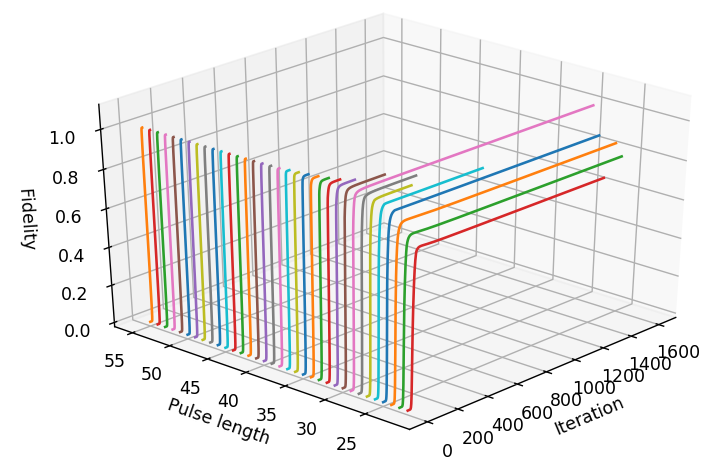
\includegraphics[width=0.7\linewidth]{figs/3d-optim-gf.png}
	\caption{Fidelity during optimizations for every pulse length (ns).}%
	\label{fig:3d-optim-gf}
\end{figure}

In \Cref{fig:fidelity-length-gf} the fidelity is shown with respect to the pulse length and it is seen that the fidelity goal is reached for pulses longer than and including \ns{30}.

\tikzfig{figs/fidelity-length-gf}{
Starting fidelity (green) and optimized fidelity (black) of pulse lengths from 22 ns to 55 ns.
}{fig:fidelity-length-gf}{0.8\textwidth}{15em}

The optimized pulses are shown in \Cref{fig:pulse_shape_gf}.
For all pulse lengths the pulses have roughly the same shape, with a quick rise and a short plateau, then oscillations until the end. 
The longest pulse at \ns{55} has more oscillations than shorter ones, but instead they are lower in amplitude.
To get some insight, the frequency spectrum, \Cref{fig:pulse_spectrum_gf}, shows large support at \(\omega_q\) and \(\omega_q+K_q\). For longer pulses, the peak at \(\omega_q-K_q\) disappears.
Just as the previous state evolution, the peaks narrow for longer pulse lengths.

\begin{figure}[ht]
\centering
\foreach \n/\capn [count=\ni] in {{22,0}/{22.0},{24,0}/{24.0},{26,0}/{26.0},{28,0}/{28.0},{29,0}/{29.0},{55,0}/{55.0}}{
	\subcaptionbox{Pulse length \capn{} ns}{
		\centering
		\setlength\figureheight{10em}
		\setlength\figurewidth{0.45\textwidth}
		\input{figs/pulse_shape_gf_\n_Real.tikz}
		\input{figs/pulse_shape_gf_\n_Imag.tikz}
	}%
	\ifnum\ni=6%
	        %
	\else%
		\hfill
	\fi%
}
\caption{Optimised pulse shapes and guess pulses (dashed) for pulse lengths 
\textbf{(a)} \SI{22}{\nano\second}, 
\textbf{(b)} \SI{24}{\nano\second}, 
\textbf{(c)} \SI{26}{\nano\second}, 
\textbf{(d)} \SI{28}{\nano\second}, 
\textbf{(e)} \SI{29}{\nano\second}, 
and \textbf{(f)} \SI{55}{\nano\second}.
Oscillations appear in all solutions.}%
\label{fig:pulse_shape_gf}
\end{figure}


\tikzfig{figs/pulse_spectrum_qubit_gf}{%
Frequency spectrum of the complex pulses in \Cref{fig:pulse_shape_gf}. The vertical lines indicate (from left to right) \(\omega_{q}-K_q\), \(\omega_{q}\), \(\omega_{q}+K_q\) (all divided by \(2\pi\)).
}{fig:pulse_spectrum_gf}{\textwidth}{18em}

The occupation dynamics in \Cref{fig:qubit_occupation_gf} show a slow oscillation for all pulse lengths for all states.
Further, the occupation probability of \(\ket{1}\) rises to about 0.75 until the middle-point of the pulse and then falls to zero in the end, while \(\ket{2}\) starts to rise at the point of the population inversion.
For the shorter pulse lengths it can be seen that there isn't enough time to realise the evolution.

\begin{figure}[ht]
\centering
\foreach \n/\capn [count=\ni] in {{22,0}/{22.0},{24,0}/{24.0},{26,0}/{26.0},{28,0}/{28.0},{29,0}/{29.0},{55,0}/{55.0}}{
	\subcaptionbox{Pulse length \capn{} ns}{
		\centering
		\setlength\figureheight{15em}
		\setlength\figurewidth{0.45\textwidth}
		\input{figs/qubit_occ_gf_\n.tikz}
	}%
	\ifnum\ni=6%
	        %
	\else%
		\hfill
	\fi%
}
\caption{Energy level occupation over time during the \(\ket{0}\rightarrow\ket{2}\) evolution for different lengths of optimized pulses.}%
\label{fig:qubit_occupation_gf}
\end{figure}

\section{Discussion}
The ``strategy'' for all pulse lengths in this case is to first invert the population and then at the halfway point start simultaneously driving the second transition level to start pumping to \(\ket{2}\).
The pulse shapes also reflects this as the oscillation that starts after the plateau has a frequency of \(K_q\), which is also visible in the frequency spectrum.
While the peak at \(\omega_q+K_q\) was expected, the peak at \(\omega_q-K_q\) for pulse lengths shorter than \ns{29} is a suprise with no clear explanation.
It is also not clear why the solutions drive harder at this frequency the shorter the pulse length.

For this optimization the initial guess pulses were very far from any solution, with the fidelity almost starting at zero for all pulse lengths.
The fidelity goal \(F > 0.99999\) was reached down to \(T = \ns{30}\), which is sightly longer than the \(\ket{0}\rightarrow\ket{1}\) evolution.
Looking at the occupation dynamics and pulse shapes could give hints as to why this is the case.
One reason could be that there needs to be enough periods of oscillations to drive to \(\ket{2}\), which is not the case for the \(\ket{0}\rightarrow\ket{1}\) evolution where the integral of the pulse shape is of importance.
Further, it appears that the fidelity drops in the same way as for the \(\ket{0}\rightarrow\ket{1}\) evolution for shorter pulse lengths.
However we cannot draw any conclusions for pulse lenghts shorter than \ns{22}.
Perhaps with a low \(\Delta F\) one might reach a solution that follows the trend, but this is only speculation.

The number of iterations also fluctuates for pulse lengths which do not reach the fidelity goal, just as for the \(\ket{0}\rightarrow\ket{1}\) evolution.

Interestingly, for both transfers the optimization converges quickly to a relatively high fidelity, while the majority of the time is spent fine-tuning the pulse shapes.
This could be a side-effect of the static step size, which could be dynamically changed for faster convergence.

To conclude, \krotov{} can also be successfully used to optimize for somewhat more complicated transfers than the simple qubit rotation.

\end{document}